\documentclass[a4paper, 12pt]{article}

\usepackage{cmap}
\usepackage{mathtext} 
\usepackage[T2A]{fontenc}
\usepackage[utf8]{inputenc}
\usepackage[english,russian]{babel}

\usepackage{amsfonts,amssymb,amsthm,mathtools}
\usepackage{amsmath}
\usepackage{icomma} 

\usepackage{graphicx} 
\graphicspath{{Picturies/}}
\usepackage{wrapfig}

\usepackage{array,tabularx,tabulary,booktabs}
\usepackage{longtable}
\usepackage{multirow}

\usepackage{caption}
\captionsetup{labelsep=period}

\renewcommand{\phi}{\varphi}
\newcommand{\eps}{\varepsilon}
\renewcommand{\AA}{\ensuremath{\mathring{A}}}
\newcommand{\parag}[1]{\paragraph*{#1:}}

\newcounter{Points}
\setcounter{Points}{1}
\newcommand{\point}{\arabic{Points}. \addtocounter{Points}{1}}

\author{Вязовцев Андрей, Б01-005}
\date{04.03.22}
\title{Лабораторная работа 4.4.1. Изучение амплитудной решётки.}

\begin {document}

\maketitle

\parag {Цель работы} знакомство с работой и настройкой гониометра Г5, определение спектральных зарактеристик амплитудной решётки.

\parag {В работе используются} гониометр, ртутная лампа, амплитудная решётка, призменный уголковый отражатель, щель с микрометрическим винтом.

\parag {Теоретическая справка} ~\\

\begin{wrapfigure}{r}{0.3\textwidth}
    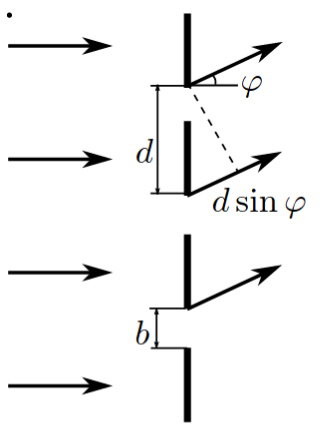
\includegraphics[scale = 0.45]{grid}
    \caption{Дифракция световой волны на амплитудной решётке\\~}
    \label{img:grid}
\end{wrapfigure}

Амплитудную решётку можно представить в виде непрозрачного экрана, в котором прорезано большое число $N$ параллельных щелей --- штрихов (см. рис. \ref{img:grid}). Постоянство расстояний между штрихами $d$ (период решётки, или шаг решётки) и шириной штриха $b$ должно выдерживаться с большой точностью.

Интенсивность дифрагированного света максимальна для углов $\phi_m$, при которых волны, приходящие в точку наблюдения от всех щелей, оказываются в фазе:

\begin{equation}
    d \sin \phi_m = m \lambda
    \label{eq:int_max}
\end{equation}

Рассмотрим изображения спектра для двух узких спектральных линий с длинами волн $\lambda$ и $\lambda + \delta \lambda$. Для минимального значения $\delta \lambda$, которое может быть определено по результатам измерений, вводят разрешающую способность:

\begin{equation}
    R = \frac{\lambda}{\delta \lambda} = \frac{\phi}{\delta \phi}
    \label{eq:R}
\end{equation}

Количество эффективно работающих штрихов и разрешающая способность связаны таким образом:

\begin{equation}
    R = m N 
    \label{eq:resolution}
\end{equation}

Найти угловую дисперсию можно так:

\begin{equation}
    D = \frac{\delta \phi}{\delta \lambda}
    \label{eq:angle_disp}
\end{equation}

\parag {Экспериментальная установка} ~

В качестве источника света используются ртутная лампа ДРШ-250. Её спектр изображён на рис. \ref{img:light}. Её характеристики указаны в таблице \ref{table:light}.

\begin{figure}[!h]
    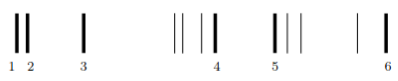
\includegraphics[scale = 1]{Workplace2}
    \centering
    \caption{Спектр ртутной лампы ДРШ-250}
    \label{img:light}
\end{figure}

\begin{table}[!h]
    \centering
    \begin{tabular}{|c|c|c|c|c|c|c|c|c|}
        \hline
        № & $К_1$ & $К_2$ & 1 & 2 & 3 & 4 & 5 & 6 \\ \hline
        $\lambda$, нм & $690,7$ & $623,4$ & $579,1$ & $577,0$ & $546,1$ & $491,6$ & $435,8$ & $404,7$ \\ \hline
        Цвет & красн. & красн. & желт. & желт. & зелен. & голуб. & синий & фиолет. \\ \hline
    \end{tabular}
    \caption {Характеристики спектра ртутной лампа ДРШ-250}
    \label{table:light}
\end{table}

Внешний вид рабочей установки изображён на рис. \ref{img:goniometr}.

\begin{figure}[!h]
    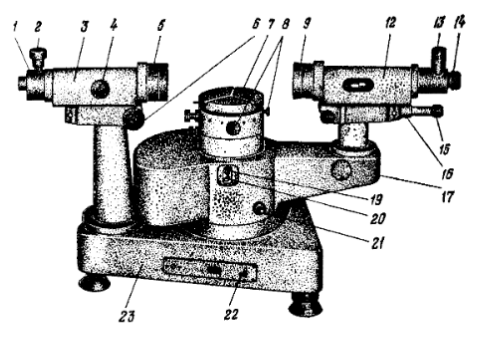
\includegraphics[scale = 1]{Workplace1}
    \centering
    \caption{Внешний вид гониометра Г5}
    \label{img:goniometr}
\end{figure}

\parag {Ход работы} ~\\

\point Настроим зрительную трубу и столик согласно методическому пособию.

\point Установим высоту входной щели так, чтобы было удобно удобно наблюдать интеренференционные полосы (т.~е. чтобы они не сливались и не были слишком тусклыми).

\point Убедимся в верности формулы \eqref{eq:int_max} при $m = \pm 1$. Например, у зелёной полосы в теории $\sin \phi = \pm 0,273$, что в точности совпадает с экспериментальным (это можно выяснить из данных, полученных далее).

\point Измерим угловые координаты спектральных линий ртути в $\pm 1$ порядках. Результаты см. в таблице \ref{table:spectr}

\begin{table}[!h]
    \centering
    \begin{tabular}{|c|c|c|c|c|}
        \hline
        цвет & красный 2 & желтый 1 & желтый 2 & зелёный \\ \hline
        $\alpha$ & $200^\circ~40'~28''$ & $199^\circ ~21'~1''$ & $199^\circ~16'~54''$ & $198^\circ ~22'~28''$ \\ \hline
        
        \multicolumn{5}{c}{ } \\ \hline
        цвет & голубой & синий & фиолетовый  & белый \\ \hline
        $\alpha$ & $196^\circ~45'~46''$ & $195^\circ ~6'~43''$ & $194^\circ~11'~58''$ & $182^\circ ~31'~50''$ \\ \hline

        \multicolumn{5}{c}{ } \\ \hline
        цвет & белый & фиолетовый & синий & голубой \\ \hline
        $\alpha$ & $182^\circ~31'~50''$ & $171^\circ ~51'~42''$ & $169^\circ~56'~56''$ & $168^\circ~18'~33''$ \\ \hline
        
        \multicolumn{5}{c}{ } \\ \hline
        цвет & зелёный & желтый 2 & желтый 1 & красный 2 \\ \hline
        $\alpha$ & $166^\circ~41'~39''$ & $165^\circ ~45'~4''$ & $165^\circ~42'~30''$ & $164^\circ ~22'~30''$ \\ \hline
    \end{tabular}
    \caption {Линии спектра ртутной лампы}
    \label{table:spectr}
\end{table}

\point Желтые линии, кроме приведённых выше, не наблюдаются.

\point Найдём угловую ширину жёлтой полосы (первой, при $m = -1$), а после выясним аппаратную разрешающую способность по формуле \eqref{eq:R}.

\begin{align*}
    \text{Левый край: }  & 199^\circ 21' 45'' \\
    \text{Правый край: } & 199^\circ 21' 3''
\end{align*}

Таким образом, $\phi = 16^\circ 49' 13''$, $\delta \phi = 42''$. 

\[
    R = \frac{\phi}{\delta \phi} \approx 1400
\]

\point Определим момент открытия щели три раза. Получаем: $0,76$ мм, $0,73$ мм, $0,73$ мм.

\point Найдём предельное разрешение по жёлтой паре первого порядка. Для это настроим щель так, чтобы пара сливалась. Получаем: $1,38$ мм.

\point Найдём количество эффективно работающих штрихов по формуле \eqref{eq:resolution}:

\[
    N = 1400
\]

Также с помощью \eqref{eq:int_max} оценим $d \approx 2$ мм (использован жёлтый максимум), что совпадает с характеристиками решётки. 

\parag {Обработка результатов} ~\\

\point Найдём $\phi_m$ для каждого максимума и построим график $\sin \phi_m (\lambda)$.

Из наклона графика ($\dfrac{\sin \phi_m}{\lambda} = (52 \pm 3) \cdot 10^{-5} ~нм^{-1}$) и формулы \eqref{eq:int_max} получаем:

\[
    d = (1.92 \pm 0.11) ~мкм
\]

Это соответствует характеристикам установки ($d = 2$ мкм).

\point Найдём угловую дисперсию по формуле \eqref{eq:angle_disp}.

\[
    D \approx  12~ \frac{угл. сек}{\AA}
\]

\point Из формулы \eqref{eq:int_max} рассчитаем порядок спектра, при котором совпадут жёлтая и фиолетовая полосы. Получим уравнение:

\[
    \lambda_{желт} m = \lambda_{фиол} (m+1)
\]

Отсюда получим:

\[
    m = \frac{\lambda_{желт}}{\lambda_{желт} - \lambda_{фиол}} \approx 2,3
\]

Но $m$ не может быть дробным. Поэтому нужно заменить $m + 1$ на $m + k$ и найти такое $k$, что $m$ близко к целому. При $k = 3$ получим $m = 7$

\begin{figure}[!h]
    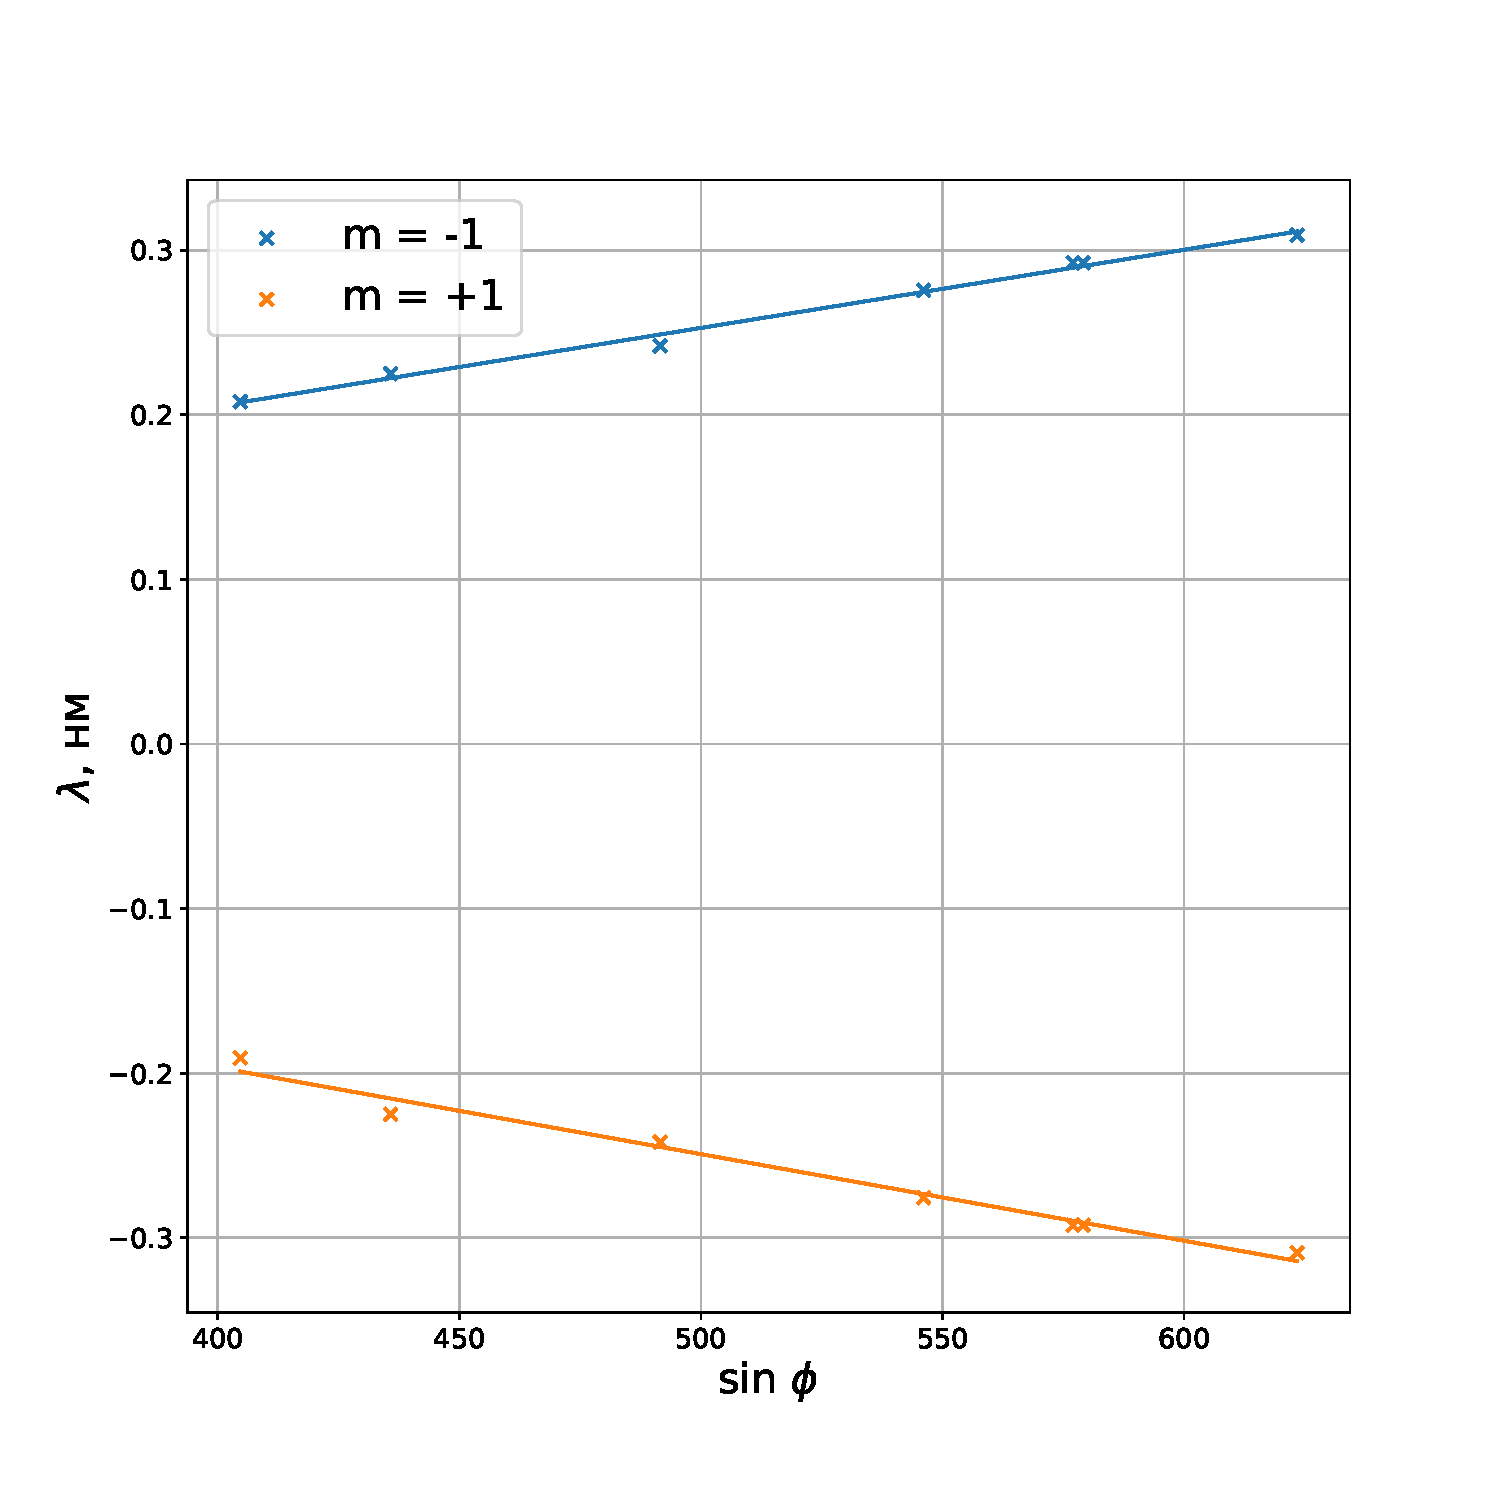
\includegraphics[scale = 0.6]{graph}
    \centering
\end{figure}

\end {document}
